\documentclass[a4paper,12pt]{article}
\usepackage{times}
\usepackage[french]{babel}
\usepackage[utf8x]{inputenc}
\usepackage[T1]{fontenc}
\usepackage{amsmath}
\usepackage{amssymb}
\usepackage{graphicx}
\usepackage{pdfpages}
\usepackage{pdflscape}
\usepackage{listings}
\usepackage{longtable}
\usepackage{hyperref}
\usepackage{graphicx} 
\graphicspath{ {./images/} }

\lstset{literate=
{é}{{\'e}}1
{è}{{\`e}}1
{ê}{{\^e}}1
{à}{{\`a}}1
{â}{{\^a}}1
}
\lstset{language=C++,
                basicstyle=\footnotesize,
                keywordstyle=\footnotesize\color{blue},
                otherkeywords={override,nullptr}
}
\definecolor{orange}{rgb}{0.8,0.4,0.0}
\definecolor{darkblue}{rgb}{0.0,0.0,0.6}
\definecolor{cyan}{rgb}{0.0,0.6,0.6}
\lstdefinelanguage{JSON}
{
  basicstyle=\normalsize,
  columns=fullflexible,
  showstringspaces=false,
  commentstyle=\color{gray}\upshape,
  morestring=[b]",
  morestring=[s]{>}{<},
  morecomment=[s]{<?}{?>},
  stringstyle=\color{orange},
  identifierstyle=\color{darkblue},
  keywordstyle=\color{blue},
  morekeywords={string,number,array,object}% list your attributes here
}

\sloppy

\setlength{\topmargin}{0cm}
\setlength{\headsep}{0.in}
\setlength{\headheight}{0.in}
\setlength{\evensidemargin}{0cm}
\setlength{\oddsidemargin}{-1cm}
\textwidth 18cm
\textheight 25cm

\begin{document}

\thispagestyle{empty}

\begin{titlepage}

\vspace*{2cm}

\begin{center}\textbf{\Huge Projet Logiciel Transversal}\end{center}{\Large \par}

\begin{center}\textbf{\large Maxime Marroufin, Quentin Chhean,\\Abinaya Mathibala, Alban Benmouffek}\end{center}{\large \par}

\vspace{2cm}

%\begin{figure}[h]
%\begin{center}
%\includegraphics[width=\textwidth]{exemple.png}
%\caption{\label{pacmangame}Exemple du jeu}
%\end{center}
%\end{figure}

\clearpage

{\small
\tableofcontents
}

\end{titlepage}

\clearpage

\section{Présentation Générale}

\subsection{Archétype}

Le jeu proposé que nous nommerons \textit{MagiX}, se base sur \href{https://en.wikipedia.org/wiki/Magic\%3A\_The_Gathering\_Online}{Magic : The Gathering Online}, la version numérique du jeu de carte à collectionner éponyme.

Dans \emph{Magic : The Gathering}, les joueurs assemblent un deck contenant $60$ cartes et s'affrontent en utilisant celles-ci.
\emph{Magic : The Gathering} est séparé en deux étapes bien distinctes : la création de deck, et le jeu en lui-même.
Nous nous focaliserons sur une seule de ces deux composantes : le jeu de carte.

\subsection{Règles du jeu}

\subsubsection{Zones de jeu}
Le Jeu est composé de sept zones :

\begin{description}
\item[La Bibliothèque :] chaque joueur a la sienne, c'est la zone ou les joueurs placent leurs deck faces cachées.
Lorsqu'un joueur pioche une carte, il pioche depuis cette zone.
\item[La Main :] propre à chaque joueur, c'est la zone depuis laquelle les joueurs peuvent jouer des cartes.
\item[Le Cimetiere :] propre à chaque joueur, c'est la zone ou les joueurs placent les cartes déffausées.
\item[L'exil :] propre à chaque joueur, c'est la zone où vont les cartes retirées du jeu par des effets de cartes.
\item[Le champ de bataille :] commun a tous les joueurs, c'est la zone ou l'on trouve des permanents qui sont soit des cartes soit des jetons crées par des effets de cartes.
\item[La Pile :] commune a tous les joueurs c'est la zone où vont les cartes jouées, effets de cartes et effets de permanents avant d'etre résolus.
\item[Zone de commandement :] commune a tous les joueurs, c'est une zone où vont des objets qui ne pourront pas être altérés par des effets de cartes.



\begin{figure}[h]
\begin{center}
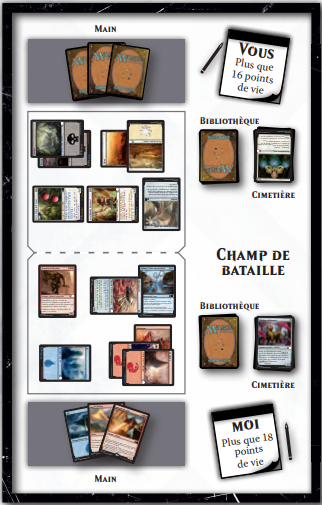
\includegraphics[width=0.6\textwidth]{Plateau.PNG}
\caption{\label{Plateau-du-jeu}Plateau du jeu}
\end{center}
\end{figure}



\end{description}

Voir exemple de plateau : Figure 1.

\subsubsection{Conditions de défaite}
Un joueur perd la partie si au moins une des conditions suivantes est réalisée : 

\begin{itemize}
\item[-] Ses points de vie sont réduits a zéro
\item[-] Il pioche alors que sa bibliothèque est vide
\item[-] Un effet de carte lui fait perdre la partie
\item[-] Un effet de carte fait gagner un de ses adversaire
\end{itemize}

\subsubsection{Structure du tour}
Le tour est composé de cinq phases.
Pendant les tours, les permanents peuvent être engagé ou dégagés.

\begin{description}
\item[Phase de début de tour :] phase pendant laquelle le joueur actif pioche une carte et dégage les permanents qu'il contrôle.
\item[Phase principale :] c'est la phase durant laquelle le joueur actif peut jouer des sorts lents.
\item[Phase de combat :] c'est la phase durant laquelle le joueur actif va déclarer une ou plusieurs créatures comme attaquant un autre joueur. Le joueur défenseur pourra alors bloquer avec ses propres créatures.
\item[Phase principale post-combat :] le joueur actif peut de nouveau jouer des sorts lents.
\item[Phase de fin de tour :] c'est la phase durant laquelle le joueur actif va défausser des cartes s'il en a trop en main et où toutes les bléssures de combats sur les créatures sont retirées.
\end{description}

\subsubsection{Déroulement de la partie}

Chaque joueur commence la partie avec un total de vingt points de vie et une main de départ de sept cartes.
La partie commence dans la phase principale du premier joueur qui joue.
À la fin de son tour, le tour d'un de ses adversaires commence.
Ce cycle continue jusqu'à ce qu'un joueur gagne la partie.

\subsection{Ressources}

\subsubsection{Textures}

Nous avons mis beaucoup de textures dans le dossier \texttt{/res/textures}.
Ces images sont libres de droit, à condition de citer la source : \href{https://www.toptal.com/designers/subtlepetterns}{Toptal Subtle Patterns}.

Nous utiliserons ces textures par exemple pour les couleurs de fond, les contours, les zones...

\subsubsection{Cartes et graphiques propres à Magic}

Les graphiques de \emph{Magic : The Gathering} ne sont pas libres de droit, on ne peut donc pas les mettre dans le dépôt Git.
À la place, nous utiliserons l'API de \href{https://scryfall.com/}{Scryfall} pour télécharger les images et les placer dans la mémoire disque des utilisaturs.

\clearpage
\section{Description et conception des états}

\subsection{Description des états}


\subsection{Conception Logiciel}


%\begin{landscape}
%\begin{figure}[p]
%
\includegraphics[width=0.9\paperheight]{state.pdf}
%\caption{\label{uml:state}Diagramme des classes d'état.} 
%\end{figure}
%\end{landscape}

\clearpage
\section{Rendu: Stratégie et Conception}

\subsection{Stratégie de rendu d'un état}


\subsection{Conception logiciel}

%\begin{landscape}
%\begin{figure}[p]
%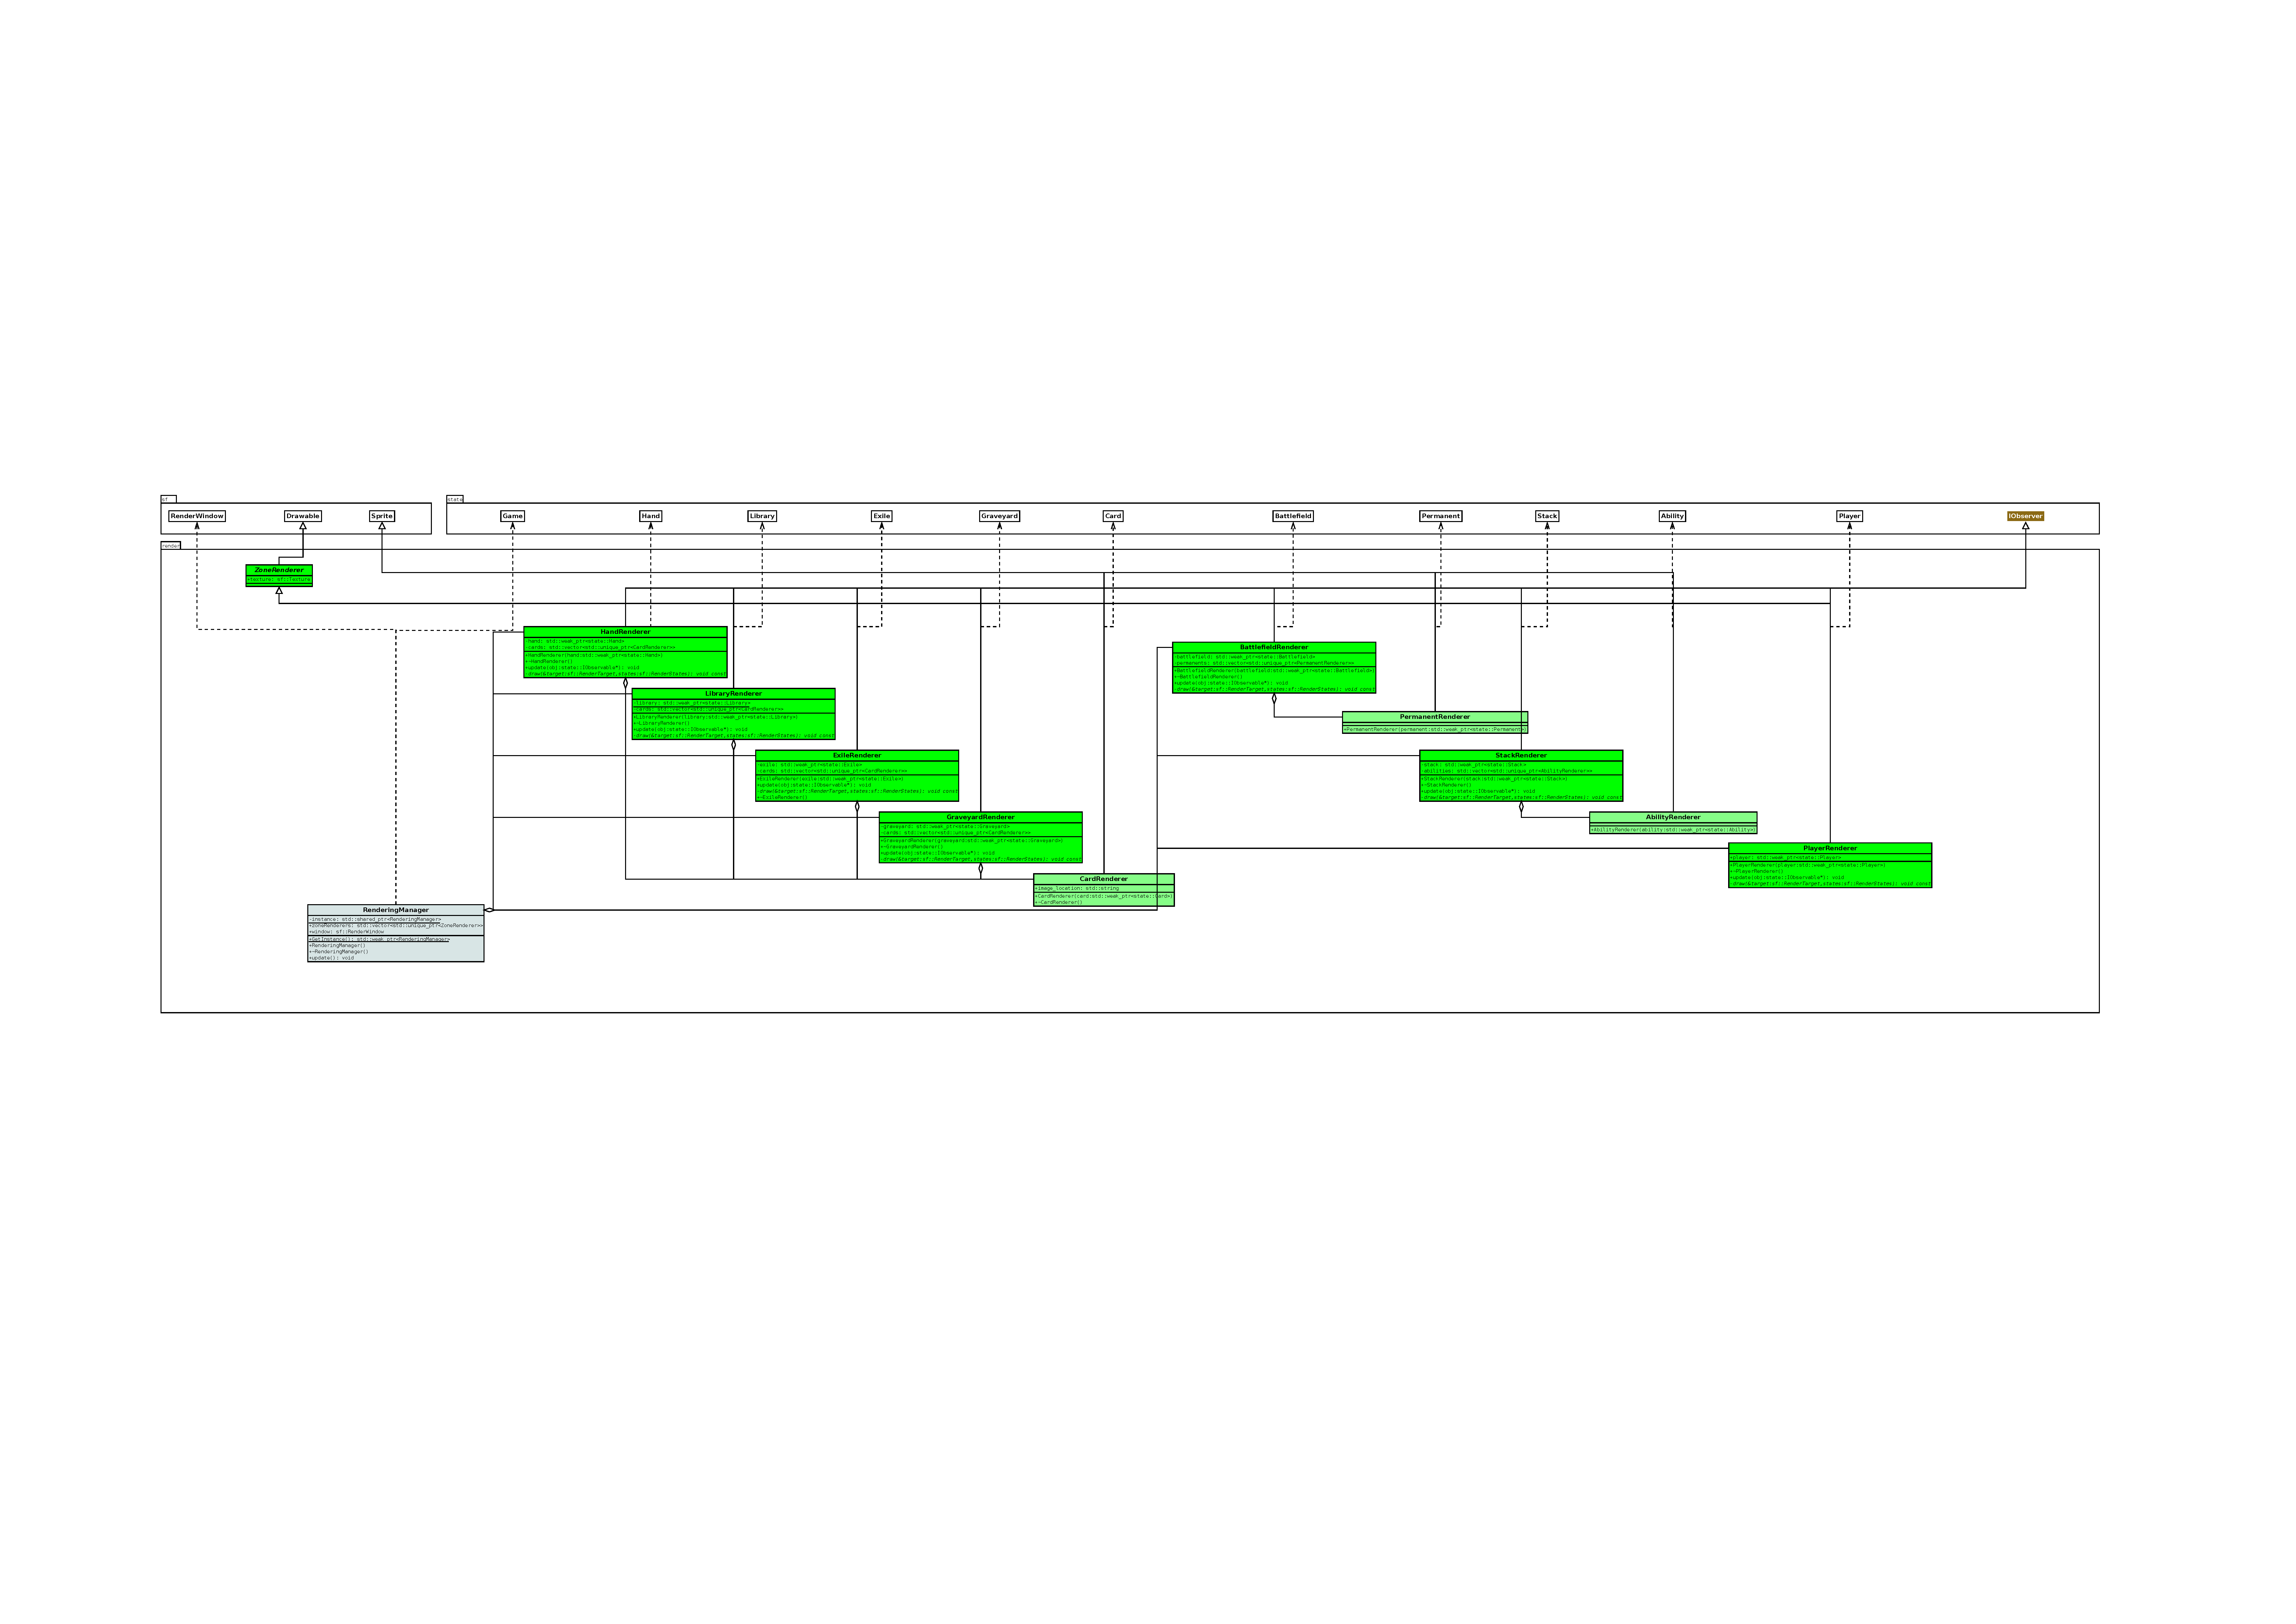
\includegraphics[width=0.9\paperheight]{render.pdf}
%\caption{\label{uml:render}Diagramme des classes de rendu.} 
%\end{figure}
%\end{landscape}

\clearpage
\section{Règles de changement d'états et moteur de jeu}

\subsection{Règles}

\clearpage
\subsection{Conception logiciel}


%\begin{landscape}
%\begin{figure}[p]
%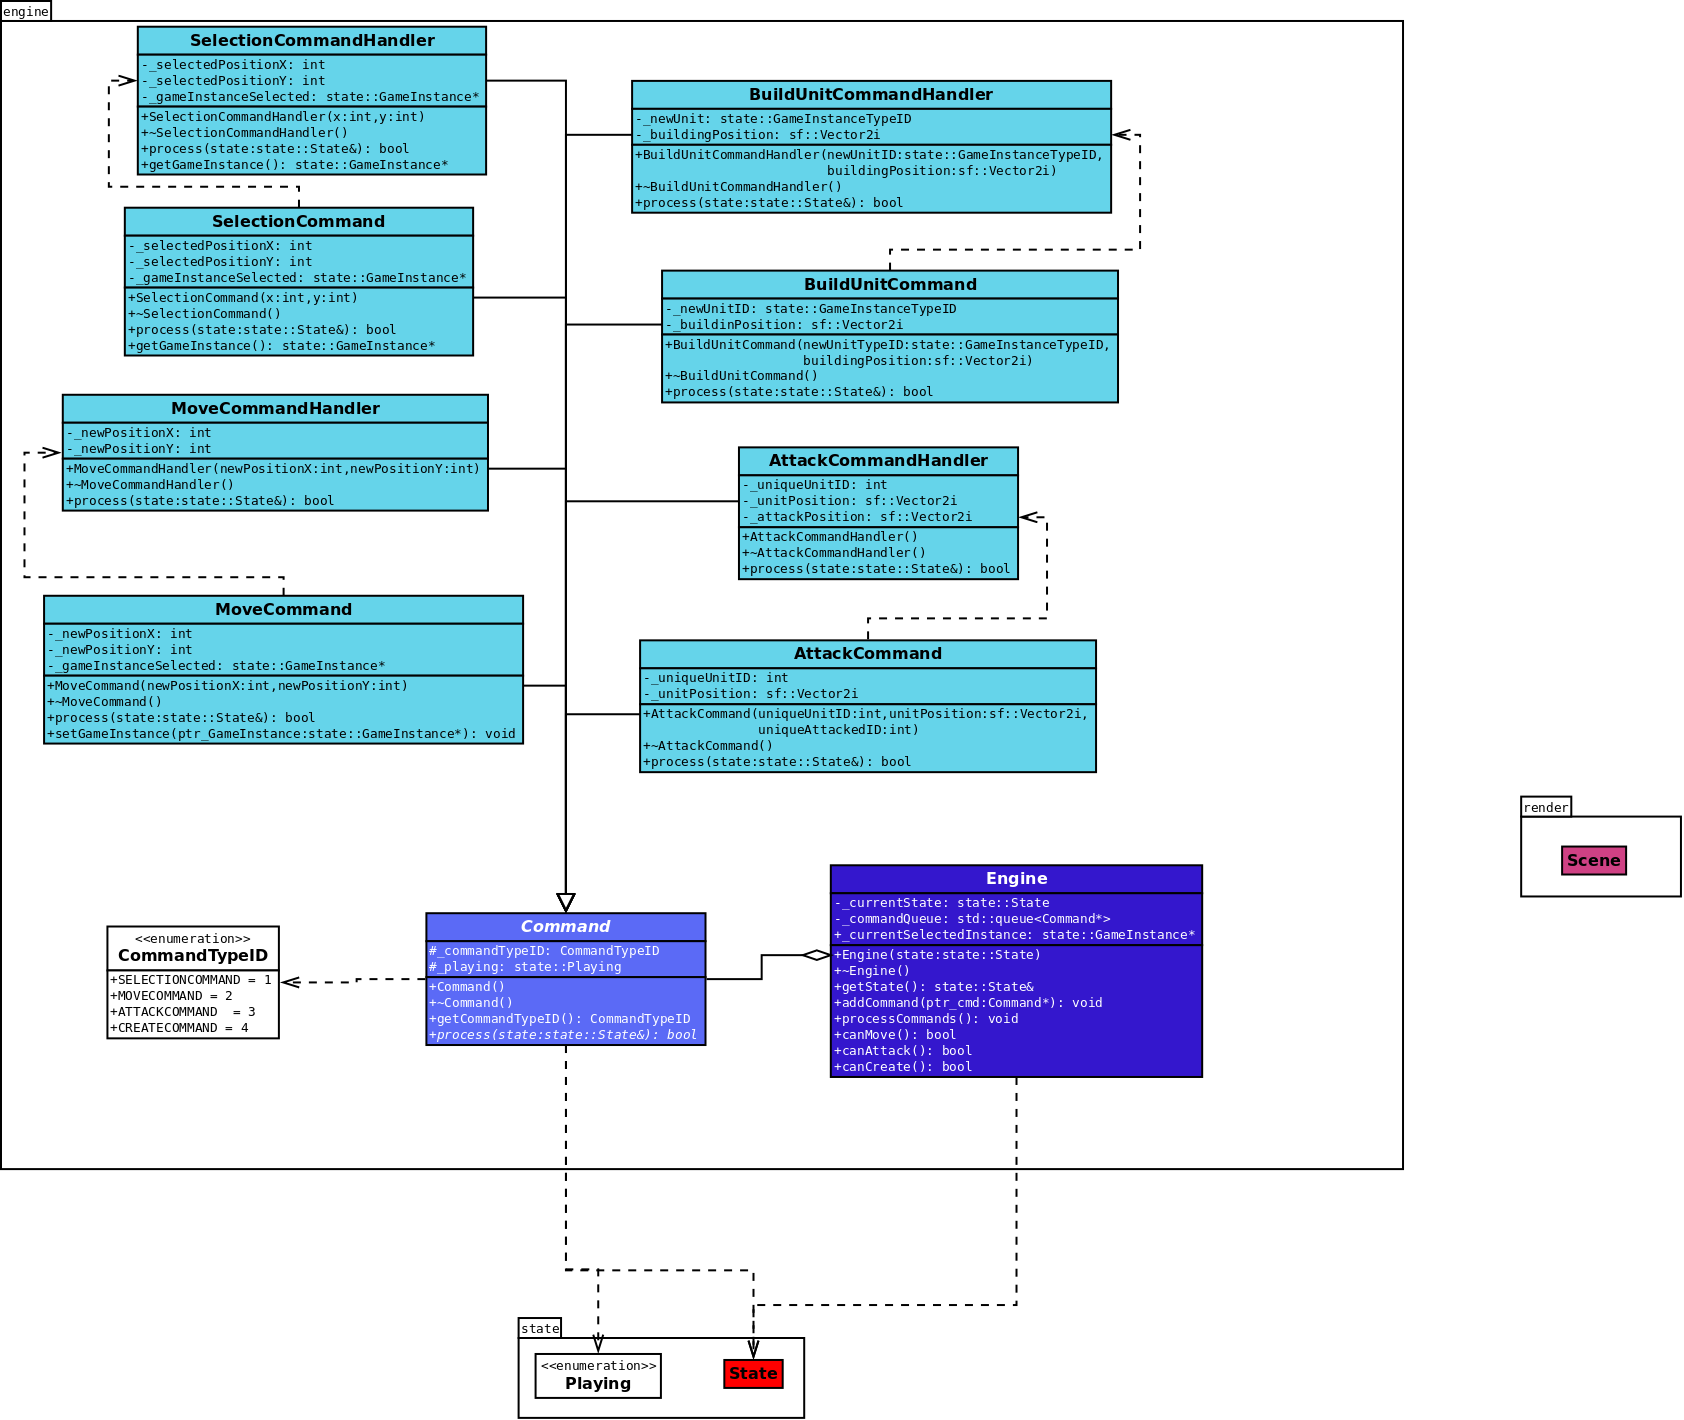
\includegraphics[width=0.9\paperheight]{engine.pdf}
%\caption{\label{uml:engine}Diagramme des classes de moteur de jeu.} 
%\end{figure}
%\end{landscape}


\section{Intelligence Artificielle}

\subsection{Stratégies}

\clearpage
\subsection{Conception logiciel}


%\begin{landscape}
%\begin{figure}[p]
%\includegraphics[width=0.9\paperheight]{ai.pdf}
%\caption{\label{uml:ai}Diagramme des classes d'intelligence artificielle.} 
%\end{figure}
%\end{landscape}


\section{Modularisation}
\label{sec:module}

\subsection{Organisation des modules}

\clearpage
\subsection{Conception logiciel}


%
%\begin{landscape}
%\begin{figure}[p]
%\includegraphics[width=0.9\paperheight]{module.pdf}
%\caption{\label{uml:module}Diagramme des classes pour la modularisation.} 
%\end{figure}
%\end{landscape}

\section{Glossaire}

\begin{description}
\item[Joueur actif :] joueur dont c'est le tour
\item[Engage/dégagé :] un permenant est dit \emph{engagé} lorsque la carte qui le représente est tournée de 90 degrés vers la droite, il est dit \emph{dégagé} lorsqu'il ne l'est pas
\item[Deck :] ensemble de cartes qu'un joueur utilise pendant la partie
\end{description}


\section{Bibliographie}

\begin{description}
\item[Règles du jeu officielles :] https://media.wizards.com/2014/docs/FR_M15_QckStrtBklt_LR_Crop.pdf

\end{description}

\end{document}
